\documentclass{beamer}

\mode<presentation>
{
  \usetheme{CambridgeUS}      % or try Darmstadt, Madrid, Warsaw, ...
  \usecolortheme{beaver} % or try albatross, beaver, crane, ...
  \usefonttheme{default}  % or try serif, structurebold, ...
  \setbeamertemplate{navigation symbols}{}
  \setbeamertemplate{caption}[numbered]
  \setbeamertemplate{theorems}[numbered]
  \setbeamertemplate{itemize items}[default]
  \setbeamertemplate{enumerate items}[default]
}

\usepackage[magyar]{babel}
\usepackage{t1enc}
\usepackage[utf8]{inputenc}
\usepackage{color}
\usepackage{amsmath}
\usepackage{amssymb}
\usepackage{enumerate}
\usepackage{tikz}
\usetikzlibrary{positioning}

\usepackage{hyperref}
\hypersetup{
    colorlinks=true,
    linkcolor=black,
    % filecolor=magenta,      
    urlcolor=cyan,
}

\setcounter{tocdepth}{1}

\title[MI a csillagászatban]{Hogyan változtatja meg a mesterséges intelligencia a csillagászatot?}
\subtitle{És úgy általában a tudományt...}
\author{Hanyecz Ottó} 
\date[MTT, \today]
{
\begin{columns}
    \begin{column}{0.9\textwidth}
        \centering
        \begin{Large}
            Polaris Csillagvizsgáló \\
        \end{Large}
        \vspace*{0.5cm}
        Budapest \\
        \vspace*{0.5cm}
        2020. október 26.
    \end{column}
\end{columns}
}

\begin{document}

\begin{frame}
    \titlepage
\end{frame}

\begin{frame}
    \frametitle{Tartalom}
    \tableofcontents
\end{frame}

\section{Big Data és mesterséges intelligencia}

\subsection{Big Data}
\begin{frame}{Mi az a Big Data?}
    \begin{columns}
        \begin{column}{0.5\textwidth}
            Large Synoptic Survey Telescope
            \begin{itemize}[<+->]
                \item Minden éjszaka feltérképezi a fél eget, ami
                \item 15 terabájt (TB) adatot termel.
                \item 10 év alatt 50 petabájt (1 PB = 1000 TB) nyers adat keletkezik,
                \item ami feldolgozva több, mint 100 PB lesz.
            \end{itemize}
            
            CERN
            \begin{itemize}[<+->]
                \item 2017. december: 1 PB adat közzététele (\href{https://home.cern/news/news/experiments/cms-releases-more-one-petabyte-open-data}{\textcolor{cyan}{CERN News}})
                \item Összesen $\sim$1,5 PB
            \end{itemize}
        \end{column}
        \begin{column}{0.5\textwidth}
            \centering
            \includegraphics[height=0.4\textheight]{figures/lsst.png} \\ %0.13
            \tiny{Fotó: LSST}

            \includegraphics[height=0.4\textheight]{figures/cms.jpg} \\ %0.25
            \tiny{Fotó: CERN/CMS}
        \end{column}
    \end{columns}
\end{frame}

\begin{frame}{Mi az a Big Data?}
    \begin{block}{Mi az a Big Data?}
        Az az adatmennyiség, amit a hagyományos adatbáziskezelők már nem tudnak kezelni, mert túl nagy, gyorsan fel kell dolgozni és sok formában létezhet.
    \end{block}
    A Big Data 4V-je:
    \begin{itemize}
        \item Volume (Mennyiség)
        \item Velocity (Sebesség)
        \item Variety (Sokféleség)
        \item Veracity (Bizonytalanság)
    \end{itemize}
\end{frame}

\begin{frame}{Big Data - problémák és a megoldás}
    Problémák:
    \begin{itemize}
        \item Nincs ember, aki lépést tud tartani ekkora adatmennyiséggel
        \item A "hagyományos" adatfeldolgozó algoritmusok túl lassúak
        \item Változó minőségű adatok
        \item Adatvizualizáció problémás lehet ($d > 3D$)
    \end{itemize}
    
    Megoldás: mesterséges intelligencia
    \begin{itemize}
        \item Minimális emberi beavatkozás kell
        \item Jó alak- és mintafelismerők
        \item Gyorsak és pontosak (de ehhez dolgozni kell)
        \item Jól kidolgozott eszközök: {\it tensorflow}, {\it keras}, {\it pandas}, {\it scikit-learn}, {\it numpy}, {\it pytorch}\dots
    \end{itemize}
\end{frame}

\subsection{A mesterséges intelligencia fogalma}
\begin{frame}{Gyenge MI vs. Erős MI}
    \begin{block}{Gyenge MI}
        \begin{itemize}
                \item Konkrét problémát old meg, de azt nagyon jól
                \item Egy konkrét algoritmussal
                \item Pl: Amazon Alexa, cicás képek azonosítása, ajánló rendszerek
            \end{itemize}
    \end{block}
    % \pause
    \centering\LARGE{$\Updownarrow$}
    % \pause
    \normalsize
    \begin{block}{Erős MI}
        \begin{itemize}
            \item Legalább olyan jól végzi el a munkát, mint az ember
            \item Általános algoritmus - {\it mindenre} jó lesz
            \item Még a közelében sem járunk
        \end{itemize}
    \end{block}
\end{frame}

\begin{frame}{Miről ismerhető fel egy szoftverben az MI?}
    \begin{itemize}
        \item<1-> A megoldandó feladat: nehéz \\
            \begin{block}{Utazó Ügynök Probléma}
                \begin{columns}
                    \begin{column}{0.5\textwidth}
                        \begin{center}
                            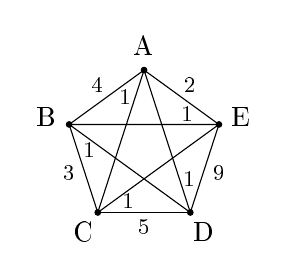
\begin{tikzpicture}
                                \foreach \x in {18,90,...,306} {
                                    \draw[fill=black,draw=black] (\x:1cm) circle [radius=1pt];
                                    \draw (\x:1cm) -- (\x+72:1cm);
                                }
                                \draw (18:1cm) -- (162:1cm)
                                      (18:1cm) -- (234:1cm)
                                      (90:1cm) -- (234:1cm)
                                      (90:1cm) -- (306:1cm)
                                      (162:1cm) -- (306:1cm);
                                \draw (90:1.3cm) node{A}
                                      (162:1.3cm) node{B}
                                      (234:1.3cm) node{C}
                                      (306:1.3cm) node{D}
                                      (18:1.3cm) node{E};
                                \draw (18+36:1cm) node{\footnotesize{2}}
                                      (90+36:1cm) node{\footnotesize{4}}
                                      (162+36:1cm) node{\footnotesize{3}}
                                      (234+36:1cm) node{\footnotesize{5}}
                                      (306+36:1cm) node{\footnotesize{9}}
                                      (18+20:0.7cm) node{\footnotesize{1}}
                                      (90+20:0.7cm) node{\footnotesize{1}}
                                      (162+20:0.7cm) node{\footnotesize{1}}
                                      (234+20:0.7cm) node{\footnotesize{1}}
                                      (306+20:0.7cm) node{\footnotesize{1}};
                            \end{tikzpicture}
                        \end{center}
                    \end{column}
                    \begin{column}{0.4\textwidth}
                        \begin{table}[h!]
                            \centering
                            \begin{tabular}{r|l}
                                Csúcs & Utak száma \\ \hline \hline
                                5 & 24 \\
                                10 & 362880 \\
                                25 & $\sim 6 \cdot 10^{23}$
                            \end{tabular}
                            % \caption{Lehetséges utak száma}
                        \end{table}
                    \end{column}
                \end{columns}
            \end{block}
        \item<2-> A szoftver viselkedése: intelligens
            \begin{itemize}
                \item Automatikus következtetés
                \item Megszerzett ismeret tárolása
            \end{itemize}
        \item<3-> Felhasznált eszközök: sajátosak
            \begin{itemize}
                \item Heurisztikával megerősített hatékony algoritmusok
                \item Gépi tanulás módszerei
            \end{itemize}
    \end{itemize}
\end{frame}

\subsection{Gépi tanulás}
\begin{frame}{Gépi tanulás}
    \begin{itemize}
        \item Egy algoritmus tanul, ha egy feladat megoldása során olyan változások következnek be a működésében, hogy később ugyanazt a feladatot jobban (eredmény, hatékonyság) képes megoldani, mint korábban
        \item Konkrét utasítások nélkül
        \item Matematikai modell készítése
        \item Felügyelt, felügyelet nélküli, megerősítéses tanulás
    \end{itemize}
\end{frame}

\begin{frame}{Felügyelt tanulás}
    \begin{itemize}
        \item {\bf Tanító minta}: a minták elvárt kimenete ismert
        % \item {\bf Tanító minta} input-output párokkal: $(x_1, y_1), (x_2, y_2), \dots (x_N, y_N)$
        %     \begin{itemize}
        %         \item Minden $y_j$ valami $y = f(x)$ ismeretlen függvényre illeszkedik
        %         \item Keresünk egy $h$ függvényt, ami a lehető legpontosabban közelíti $f$-t
        %     \end{itemize}
        \item {\bf Teszt mintával} ellenőrizzük az illesztés pontosságát
        % \item Műkedvelőknek: $$\min \frac{1}{N} \sum_{n=1}^{N} \mathcal{L}(f(\Theta, x_n), y_n)$$
        \item Két nagy csoport: osztályozás és regresszió (előrejelzés)
        \item Példák: időjárás-előrejelzés, népességnövekedés, kép és spam felismerése (Feladat: melyik példa melyik csoportba tartozik?)
    \end{itemize}
\end{frame}

\begin{frame}{Felügyelt tanulás - Várjunk-e az asztalra?}
    \centering
    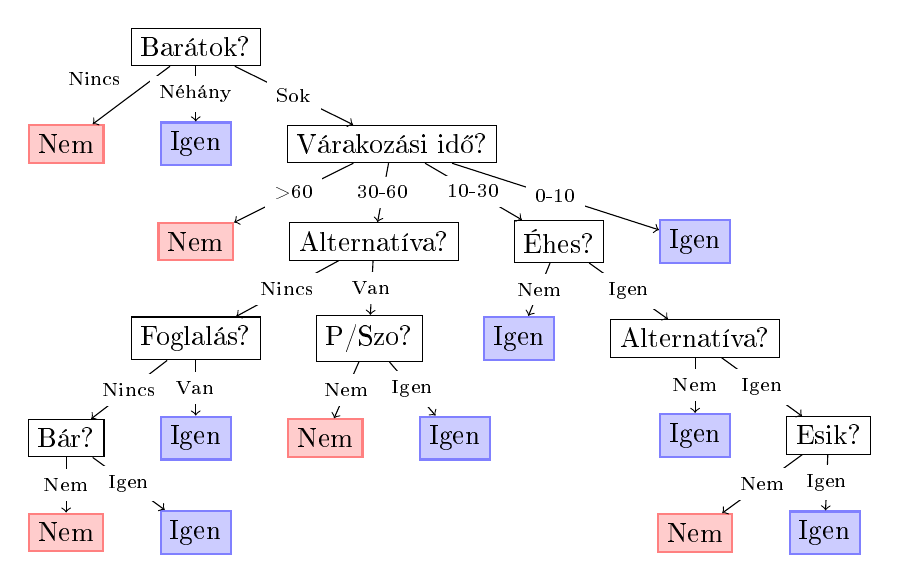
\begin{tikzpicture}
        [no/.style={rectangle,draw=red!50,fill=red!20,thick},
         yes/.style={rectangle,draw=blue!50,fill=blue!20,thick},
         question/.style={rectangle,draw},
         every node/.style={node distance=7mm},
         dec/.style={midway,fill=white}]
        
        \node[no] (n1) {Nem};
        \node[yes] (y1) [right=of n1] {Igen};
        \node[question] (q1) [above=of y1] {Barátok?}
            edge [->] node[auto,swap] {\scriptsize Nincs}   (n1)
            edge [->] node[dec]      {\scriptsize Néhány}  (y1);
        
        % Várakozási idő és annak gyerekei
        \node[no]       (n2) [below=of y1] {Nem};
        \node[question] (q2) [right=of y1] {Várakozási idő?}
            edge [<-] node[dec] {\scriptsize Sok} (q1)
            edge [->] node[dec] {\scriptsize >60} (n2);
            
        \node[question] (q3) [right=of n2] {Alternatíva?}
            edge [<-] node[dec] {\scriptsize 30-60} (q2);
            
        \node[question] (q4) [right=of q3] {Éhes?}
            edge [<-] node[dec] {\scriptsize 10-30} (q2);
        
        \node[yes] (y2) [right=of q4] {Igen}
            edge [<-] node[dec] {\scriptsize 0-10} (q2);
        
        % Alternatíva és Éhes gyerekei
        \node[question] (q5) [below=of n2] {Foglalás?}
            edge [<-] node[dec] {\scriptsize Nincs} (q3);
        \node[question] (q6) [right=of q5] {P/Szo?}
            edge [<-] node[dec] {\scriptsize Van} (q3);
        \node[question] (q7) [below=of y2] {Alternatíva?}
            edge [<-] node[dec] {\scriptsize Igen} (q4);
        \node[yes] (y3) [left=of q7] {Igen}
            edge [<-] node[dec] {\scriptsize Nem} (q4);
        
        % Foglalás és P/Szo gyerekei
        \node[yes] (y4) [below=of q5] {Igen}
            edge [<-]node[dec] {\scriptsize Van} (q5);
        \node[question] (q8) [left=of y4] {Bár?}
            edge [<-] node[dec] {\scriptsize Nincs} (q5);
        \node[no] (n3) [right=of y4] {Nem}
            edge [<-] node[dec] {\scriptsize Nem} (q6);
        \node[yes] (y5) [right=of n3] {Igen}
            edge [<-] node[dec] {\scriptsize Igen} (q6);
            
        % Bár gyerekei
        \node[no] (n4) [below=of q8] {Nem}
            edge [<-] node[dec] {\scriptsize Nem} (q8);
        \node[yes] (y5) [right=of n4] {Igen}
            edge [<-] node[dec] {\scriptsize Igen} (q8);
        
        % Alternatíva gyerekei
        \node[yes] (y6) [below=of q7] {Igen}
            edge [<-] node[dec] {\scriptsize Nem} (q7);
        \node[question] (q9) [right=of y6] {Esik?}
            edge [<-] node[dec] {\scriptsize Igen} (q7);
        \node[no] (n5) [below=of y6] {Nem}
            edge [<-] node[dec] {\scriptsize Nem} (q9);
        \node[yes] (y8) [right=of n5] {Igen}
            edge [<-] node[dec] {\scriptsize Igen} (q9);
    \end{tikzpicture}
\end{frame}


\begin{frame}{Nemfelügyelt tanulás}
    \begin{itemize}
        \item Tanító minta csak input adatokkal - nem ismert, hogy az adat micsoda
        \item Úgy csoportosítunk, hogy a hasonlók egy csoportba kerüljenek
    \end{itemize}
    
    \centering
    \begin{tikzpicture}
        \node<1> (img1) {\includegraphics[scale=0.25]{figures/k-means-1.png}};
        \node<2> (img2) {\includegraphics[scale=0.25]{figures/k-means-2.png}};
        \node<3> (img3) {\includegraphics[scale=0.25]{figures/k-means-3.png}};
        \node<4> (img4) {\includegraphics[scale=0.25]{figures/k-means-4.png}};
        \node<5> (img5) {\includegraphics[scale=0.25]{figures/k-means-5.png}};
        \node<6> (img6) {\includegraphics[scale=0.25]{figures/k-means-6.png}};
        
        % \node<7> (img7) {\includegraphics[scale=0.6]{figures/color1.png}};
        % \node<8> (img8) {\includegraphics[scale=0.6]{figures/color2.png}};
        % \node<9> (img9) {\includegraphics[scale=0.6]{figures/color3.png}};
    \end{tikzpicture}
\end{frame}

\begin{frame}{Megerősítéses tanulás}
    \begin{itemize}
        % \item Példa: \href{https://deepmind.com/research/case-studies/alphago-the-story-so-far}{AlphaGo} (2015 október, 5-0)
        \item Példa:
        \begin{itemize}
            \item \href{https://www.youtube.com/watch?v=VMp6pq6_QjI}{AI Learns to Park (Youtube)}
            \item \href{https://www.youtube.com/watch?v=CqYKhbyHFtA}{Two AI Fight for the same parking spot (Youtube)}
        \end{itemize}
        \item Nincs visszajelzés, hogy mi a jó vagy rossz
        \item Az algoritmus {\it megtanulja}, hogy melyik a jó lépés
        \item Mi lehet megerősítés? Mikor kap az algoritmus megerősítést?
    \end{itemize}
\end{frame}

\subsection{Neurális hálók}

\begin{frame}{Neurális hálók}
    \centering
    \begin{tikzpicture}
        \node<1> (img1) {\includegraphics[scale=0.34]{figures/neuron.png}};
        \node<2> (img2) {\includegraphics[scale=0.34]{figures/neuron-model.png}};
    \end{tikzpicture}
\end{frame}

\begin{frame}{Neurális hálók}
    Első matematikai leírás: McCulloch and Pitts (1943)
    
    \centering
    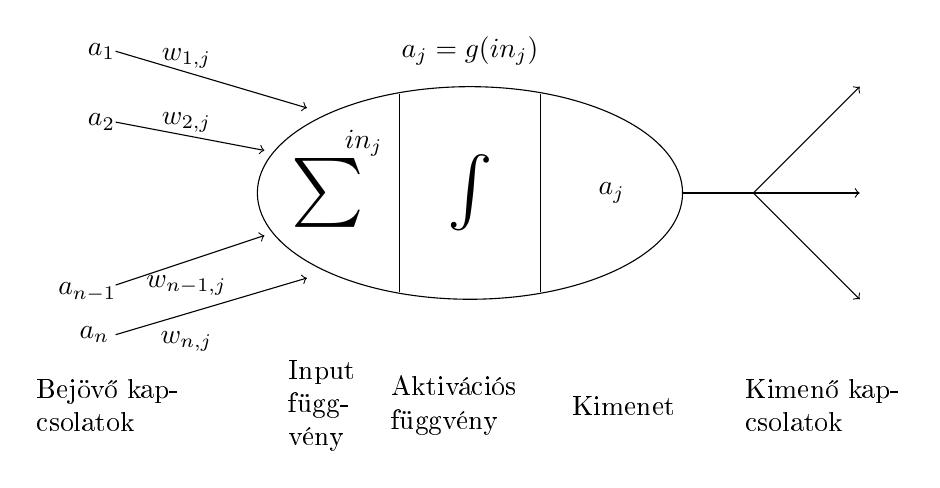
\begin{tikzpicture}[scale=0.9]
        \draw[->] (-5,2) -- (-2.3,1.2);
        \draw[->] (-5,1) -- (-2.9,0.6);
        \draw[->] (-5,-1.3) -- (-2.9,-0.6);
        \draw[->] (-5,-2) -- (-2.3,-1.2);
        \draw (-5.2,2) node{$a_1$};
        \draw (-5.2,1) node{$a_2$};
        \draw (-5.4,-1.4) node{$a_{n-1}$};
        \draw (-5.3,-2) node{$a_n$};
        \draw (-4,1.9) node{$w_{1,j}$};
        \draw (-4,1) node{$w_{2,j}$};
        \draw (-4,-1.3) node{$w_{n-1,j}$};
        \draw (-4,-2.1) node{$w_{n,j}$};
        
        \draw (0,0) ellipse [x radius=3cm, y radius=1.5cm];
        \draw (-2,0) node{\Huge{$\sum$}};
        \draw (-1.5,0.7) node{$in_j$};
        \draw (-1,1.4) -- (-1,-1.4);
        \draw (0,0) node{\Huge{$\int$}};
        \draw (1,1.4) -- (1,-1.4);
        \draw (2,0) node{$a_j$};
        \draw (0,2) node{$a_j=g(in_j)$};
        
        \draw (3,0) -- (4,0);
        \draw[->] (4,0) -- (5.5,1.5);
        \draw[->] (4,0) -- (5.5,0);
        \draw[->] (4,0) -- (5.5,-1.5);
        \draw (-5,-3) node[text width=2cm]{Bejövő kapcsolatok};
        \draw (-2,-3) node[text width=1cm]{Input függvény};
        \draw (0,-3) node[text width=2cm]{Aktivációs függvény};
        \draw (2,-3) node[text width=1cm]{Kimenet};
        \draw (5,-3) node[text width=2cm]{Kimenő kapcsolatok};
    \end{tikzpicture}
\end{frame}

\begin{frame}{Neurális hálók - aktivációs függvények}
    \hspace*{-1.5cm}
    \includegraphics[width=1.23\textwidth]{figures/activation_functions.pdf} \\
    ReLU = rectified linear units
\end{frame}

\begin{frame}{Neuráis hálók - Feed-forward háló}
    \centering
    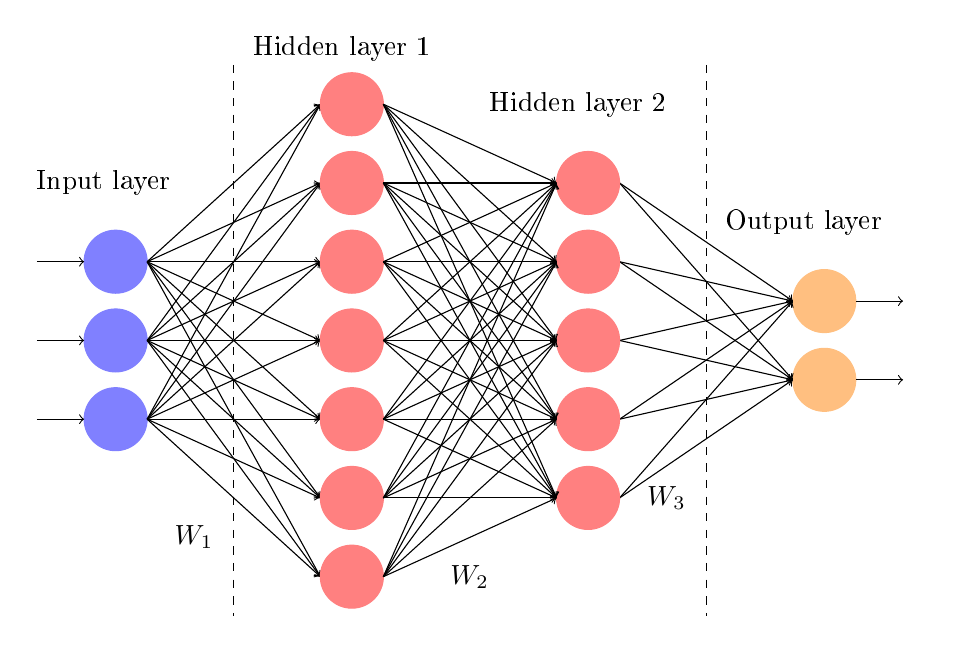
\begin{tikzpicture}
        % Input layer
        \foreach \y in {-1,0,1} {
            \draw[draw=blue!50,fill=blue!50] (-3, \y) circle [radius=0.4cm];  % Neuronok
            \draw[->] (-4, \y) -- (-3.4, \y);          % Inputba menő nyilak
            
            % Első hidden layer-be menő nyilak
            \foreach \yy in {-3,-2,-1,0,1,2,3} {
                \draw[->] (-2.6, \y) -- (-0.4, \yy);
            }
        }
        
        % Output layer
        \foreach \y in {0.5,-0.5} {
            \draw[draw=orange!50,fill=orange!50] (6,  \y) circle [radius=0.4cm];  % Neuronok
            \draw[->] (6.4, \y) -- (7, \y);            % Output-ból kimenő nyilak
            
            % Output layer-be menő nyilak
            \foreach \yy in {-2,-1,0,1,2} {
                \draw[->] (3.4, \yy) -- (5.6, \y);
            }
        }
        
        % Hidden layer 1
        \foreach \y in {-3,-2,-1,0,1,2,3} {
            \draw[draw=red!50,fill=red!50] (0, \y) circle [radius=0.4cm];
        }
        
        % Hidden layer 2
        \foreach \y in {-2,-1,0,1,2} {
            \draw[draw=red!50,fill=red!50] (3, \y) circle [radius=0.4cm];
        }
        
        % Hidden layer-ek közötti nyilak
        \foreach \y in {-3,-2,-1,0,1,2,3} {
            \foreach \yy in {-2,-1,0,1,2} {
                \draw[->] (0.4, \y) -- (2.6, \yy);
            }
        }
        
        % Feliratok
        \draw (-3,   2)   node[text width=2cm]   {Input layer};
        \draw ( 0,   3.7) node[text width=2.5cm] {Hidden layer 1};
        \draw ( 3,   3)   node[text width=2.5cm] {Hidden layer 2};
        \draw ( 6,   1.5) node[text width=2.5cm] {Output layer};
        \draw (-1,  -2.5) node[text width=2.5cm] {$W_1$};
        \draw ( 2.5,-3)   node[text width=2.5cm] {$W_2$};
        \draw ( 5.,-2)   node[text width=2.5cm] {$W_3$};
        
        % Elválasztó vonalak
        \draw[dashed] (-1.5, 3.5) -- (-1.5, -3.5);
        \draw[dashed] ( 4.5, 3.5) -- ( 4.5, -3.5);
    \end{tikzpicture}
\end{frame}


\begin{frame}{Neurális hálók}
    Problémák:
    \begin{itemize}
        \item Nincs általános háló
        \item Próbálgatással kell a jó hálót beállítani (vagy ügyesen megsejteni)
        \item Feed-forward hálók nem foglalkoznak a bemenet térbeli felépítésével
        \item Mennyi 
    \end{itemize}
    
    Megoldás: 
    \begin{itemize}
        \item Mély neurális hálók
        \item Konvolúciós neurális hálók
        \item Generatív modellek
    \end{itemize}
\end{frame}




\end{document}
